% \title{Apunte de Matemáticas Discretas CC3101:\\ 
% Conceptos básicos sobre grafos  Clase 17}
% % \title{Ejercicios Lógica e Inducción}
% \author{Andrés Abeliuk}
% \date{}
% \maketitle

\section{Introducción a los Grafos}

\subsection{Motivación y Aplicaciones}
% \begin{center}
% \begin{tikzpicture}[scale=0.8, transform shape, every node/.style={circle, draw, fill=white, minimum size=0.7cm}]
% \node (A) at (0,0) {A};
% \node (B) at (2,2) {B};
% \node (C) at (2,0) {C};
% \node (D) at (1,-1.5) {D};
% \node (E) at (4,0) {E};
% \node (F) at (5,2) {F};
% \node (G) at (5,-1.5) {G};

% \draw (A) -- (B);
% \draw (A) -- (C);
% \draw (A) -- (D);
% \draw (B) -- (C);
% \draw (C) -- (D);
% \draw (C) -- (E);
% \draw (E) -- (F);
% \draw (E) -- (G);
% \end{tikzpicture}
% \end{center}
Los grafos son estructuras matemáticas utilizadas para modelar relaciones entre objetos. Son fundamentales en ciencias de la computación, matemática discreta, teoría de redes, y muchas otras disciplinas.

\begin{definitionblock}{Definición: Grafo}
Un \emph{grafo} $G = (V,E)$ está compuesto por un conjunto no vacío $V$ de vértices (o nodos) y un conjunto $E$ de aristas (o arcos) que conectan pares de vértices.
\end{definitionblock}
\noindent\textbf{Notación:} Usaremos $(v_1,v_2)$ para denotar una arista (o arco) entre los nodos $v_1$ y $v_2$, donde $v_1, v_2 \in V$. Esta notación también será válida para representar la dirección en el caso de grafos dirigidos.



\subsection{Historia}
\begin{exampleblock}{Historia: Los Puentes de Königsberg}
El matemático Leonhard Euler resolvió en 1736 el famoso problema de los puentes de Königsberg, una ciudad atravesada por un río y dividida en varias islas conectadas por siete puentes. El desafío consistía en encontrar un recorrido que cruzara cada puente exactamente una vez.\\

Para abordar el problema, Euler realizó una abstracción revolucionaria: representó cada porción de tierra como un nodo y cada puente como una arista que conecta dos nodos. Esta representación marcó el nacimiento formal de la teoría de grafos.\\

Su demostración mostró que no es posible recorrer todos los puentes sin repetir alguno, y estableció principios fundamentales sobre conectividad y estructura. La enseñanza clave es que muchos problemas complejos se simplifican cuando se modelan como grafos.
\end{exampleblock}
\begin{center}
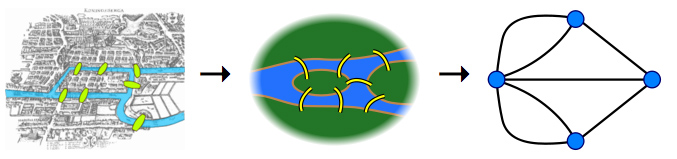
\includegraphics[width=0.9\textwidth]{Figures/bridges.jpg} \\
\smallskip
\small{\textit{Abstracción del problema de los Puentes de Königsberg: desde el mapa original hasta su representación como grafo.}} \
\href{https://en.wikipedia.org/wiki/File:Konigsberg_bridges.png}{\scriptsize{Imagen: Bogdan Giuşcă.}}
\end{center}

\subsection{Ejemplos de aplicaciones}
Los grafos no solo son una herramienta matemática elegante, sino también un lenguaje poderoso para representar sistemas complejos en el mundo real. A continuación, se presentan algunas aplicaciones concretas y ampliamente estudiadas del uso de grafos en distintas áreas del conocimiento y la tecnología \footnote{Barabási, A.-L. (2016). \href{http://networksciencebook.com/}{\textit{Network Science}}. Cambridge University Press.} 

\begin{itemize}
\item Modelar redes de comunicación: cada dispositivo es un nodo, y una conexión directa entre dos dispositivos (como un cable o enlace inalámbrico) se modela como una arista. Esto permite representar arquitecturas de red como topologías en estrella, anillo o malla, facilitando el análisis de eficiencia y tolerancia a fallos.

\item Representar relaciones sociales: personas como nodos y las amistades, interacciones o vínculos (como seguir a alguien en redes sociales) como aristas. Esta abstracción permite estudiar propiedades como centralidad, comunidades, y difusión de información.

\item Representar colaboraciones científicas: se construyen grafos donde cada nodo es un autor, y dos autores están conectados si han publicado juntos. Un ejemplo contemporáneo es el uso de bases de datos académicas para modelar la evolución de la colaboración interdisciplinaria.

\item Modelar el transporte: estaciones, paraderos o aeropuertos son nodos, y las rutas (como líneas de metro, vuelos o carreteras) son aristas. Esto permite optimizar rutas, estudiar congestión o conectividad.
\end{itemize}






\subsection{Clasificación de Grafos}

\subsection*{Tipos de grafos}
\begin{itemize}
\item \textbf{Grafo simple}: sin lazos ni aristas paralelas.
\item \textbf{Multigrafo}: permite aristas paralelas.
\item \textbf{Grafo con lazos}: permite aristas de un nodo a sí mismo.
\item \textbf{Grafos dirigidos}: las aristas tienen dirección.
\end{itemize}

\begin{center}
\begin{tabular}{lccc}
\toprule
\textbf{Nombre} & \textbf{Aristas} & \textbf{Aristas paralelas} & \textbf{Lazos} \\
\midrule
Grafo simple & No dirigidas & No & No \\
Multigrafo & No dirigidas & Sí & No \\
Grafo & No dirigidas & Sí & Sí \\
Grafo dirigido simple & Dirigidas & No & No \\
Multigrafo dirigido & Dirigidas & Sí & No \\
Grafo dirigido & Dirigidas & Sí & Sí \\
\bottomrule
\end{tabular}
\end{center}

\subsection{Terminología}

\subsubsection*{Grafos no dirigidos}
\begin{itemize}
\item Dos nodos son \textbf{adyacentes} si comparten una arista.
\item Una arista es \textbf{incidente} a un nodo si el nodo es uno de sus extremos.
\item El \textbf{grado} de un nodo $v$, denotado $\deg(v)$, es el número de aristas incidentes (los lazos cuentan doble).
\item Un nodo es \textbf{aislado} si $\deg(v) = 0$.
\end{itemize}

\subsubsection*{Grafos dirigidos}
\begin{itemize}
\item En una arista $(u,v)$, $u$ es el \textbf{origen} y $v$ el \textbf{destino}.
\item \textbf{Grado de entrada}: $\deg^{-}(v)$ es el número de aristas que llegan a $v$.
\item \textbf{Grado de salida}: $\deg^{+}(v)$ es el número de aristas que salen de $v$.
\end{itemize}




\subsection{Ejemplos empíricos: Distribución de grado en redes reales}
Una propiedad estructural fundamental de un grafo es su \textbf{distribución de grado}, que indica cuántos nodos tienen $k$ conexiones para cada posible valor de $k$. Esta distribución revela la organización global de la red y es especialmente importante en grafos grandes como los que aparecen en contextos reales.

En la siguiente figura se observan distribuciones de grado para diferentes redes reales, muchas de las cuales exhiben comportamientos que siguen una ley de potencias:

\begin{center}
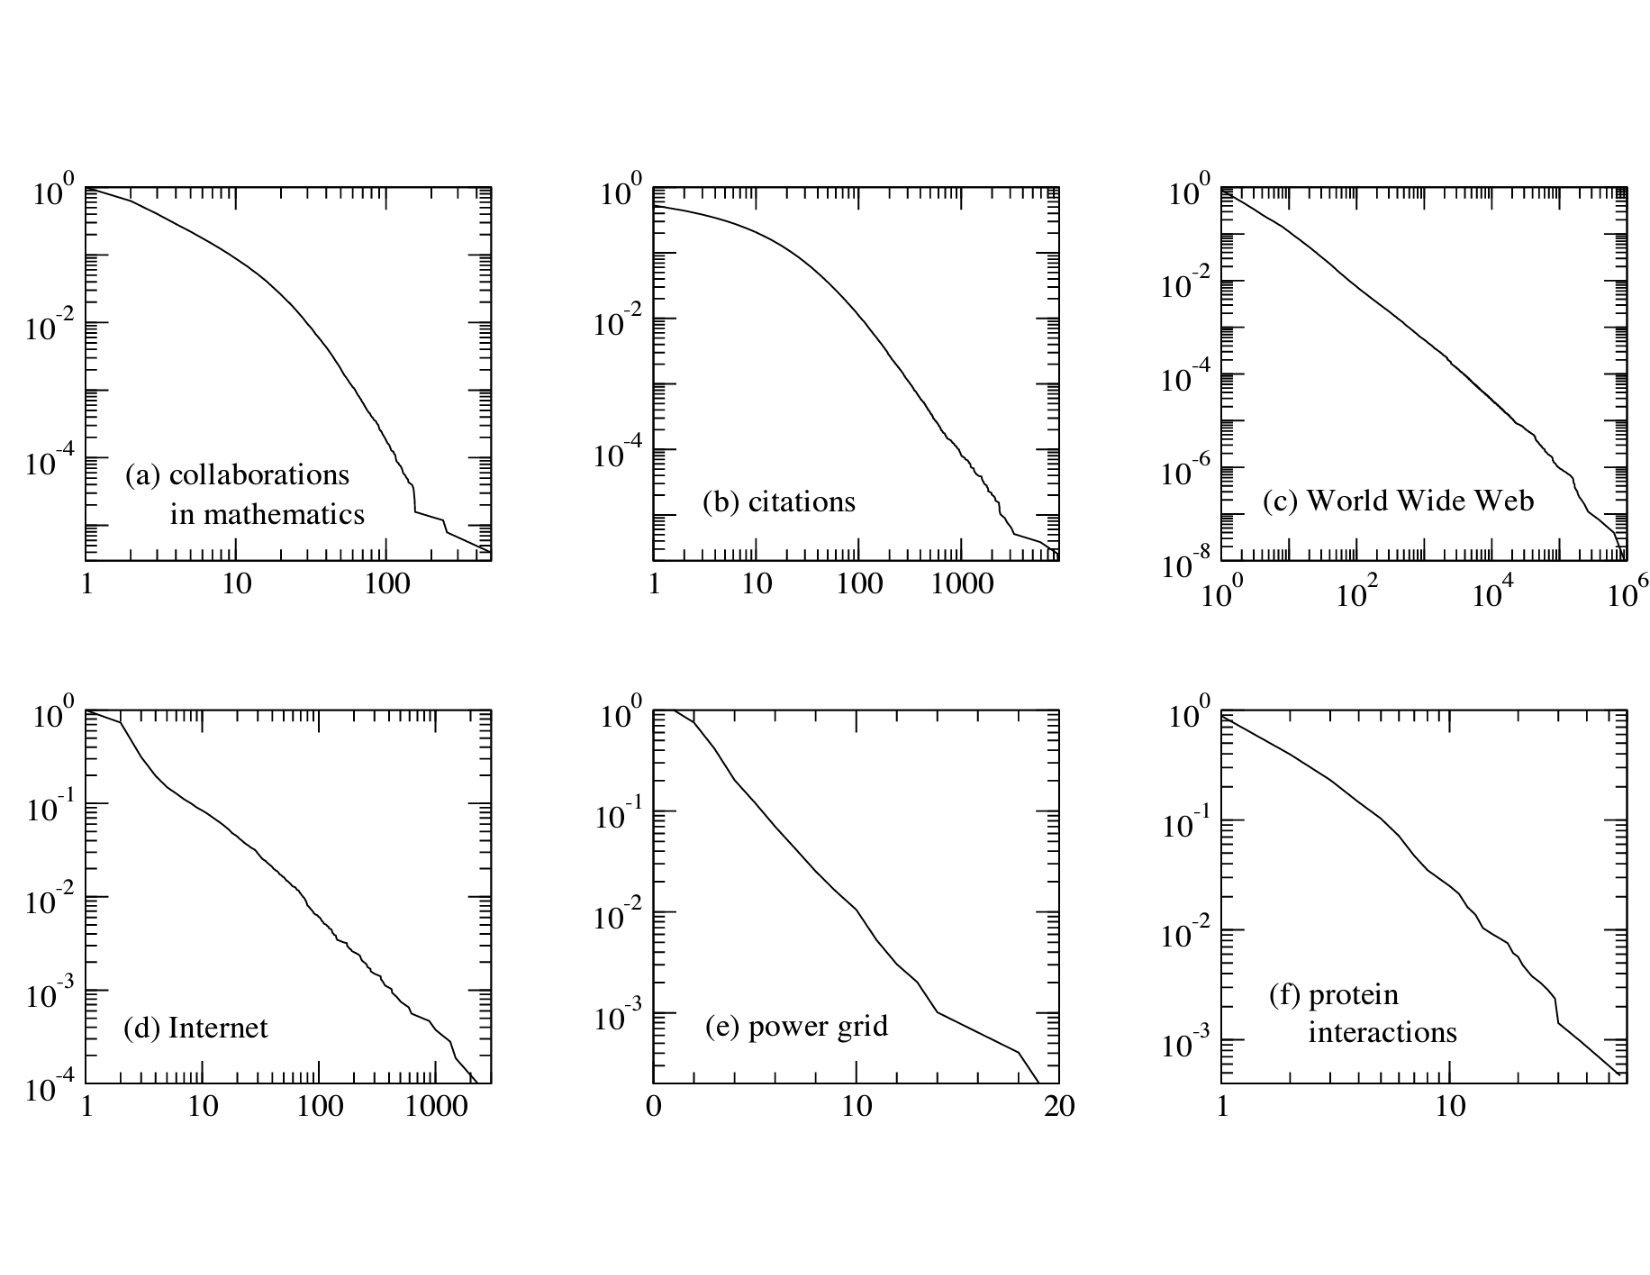
\includegraphics[width=0.8\textwidth]{Figures/power_law.pdf} \\
\small{\textit{Distribuciones de grado para diversas redes: colaboración matemática, citas, web, internet, red eléctrica y proteínas.}} 
\scriptsize{Fuente: Newman, M.E.J. (2003). \href{https://doi.org/10.1137/S003614450342480}{\textit{The Structure and Function of Complex Networks}}. \textit{SIAM Review}.}
\end{center}

\subsection*{Características comunes}

\begin{itemize}
\item En redes como la web, el internet o las redes sociales, la mayoría de los nodos tiene pocos enlaces, mientras que unos pocos tienen muchos (nodos \emph{hub}).
\item Este comportamiento es típico de una \textbf{distribución de grado sesgada} o de tipo \emph{escala libre}, en contraste con una red aleatoria.
\item En estos casos, la probabilidad de que un nodo tenga grado $k$ decrece como $P(k) \sim k^{-\gamma}$ para alguna constante $\gamma$.
\end{itemize}

Estas propiedades tienen consecuencias importantes: los hubs pueden facilitar la difusión rápida de información o infecciones, pero también pueden ser puntos vulnerables si fallan.




\section{Propiedades de los Grafos}
Una de las propiedad de los grafos no dirigidos es la relación entre el número total de aristas y los grados de los vértices. Esta relación se conoce comúnmente como el \emph{Teorema de los saludos}, ya que puede interpretarse en un contexto cotidiano: 
El número total de apretones de manos en una fiesta es igual a la suma de las manos estrechadas por cada persona, y por lo tanto, siempre es par. En consecuencia, el número de personas que da un número impar de apretones es par.

\begin{thmblock}{Teorema de los saludos}
Sea $G = (V, E)$ un grafo no dirigido. Entonces:
$$
\sum_{v \in V} \deg(v) = 2|E|
$$
En particular, \textbf{el número de nodos de grado impar es par}.
\end{thmblock}

\begin{proof}
El resultado es inmediato ya que cada arista $e \in E$ aporta dos unidades
a la suma $\sum_{v \in V} deg(v)$. (Puede probarse más
formalmente haciendo inducción sobre el número de aristas del grafo.)

\medskip

Para probar que el número de nodos de grado impar es par, consideremos la suma total $S = \sum_{v \in V} \deg(v)$ como una suma de enteros. Dado que $S$ es par (igual a $2|E|$), y que la suma de números impares sólo puede ser par si hay una cantidad par de sumandos impares, se deduce que debe haber un número par de vértices con grado impar.
\end{proof}

% \begin{exampleblock}{Ejemplo}
% Considere un grafo con $5$ vértices y $4$ aristas:
% \begin{itemize}
% \item $\deg(v_1) = 2$, $\deg(v_2) = 1$, $\deg(v_3) = 2$, $\deg(v_4) = 1$, $\deg(v_5) = 2$.
% \end{itemize}
% Entonces:

% Además, los vértices $v_2$ y $v_4$ tienen grado impar, y hay exactamente dos de ellos.
% \end{exampleblock}

\begin{thmblock}{Lema de grados para grafos dirigidos}
Sea $G=(V,E)$ un grafo dirigido. Entonces:

$$
\sum_{v \in V} \deg^{-}(v) = \sum_{v \in V} \deg^{+}(v) = |E|
$$
\end{thmblock}

\begin{proof}
Cada arista dirigida $(u,v) \in E$ tiene un nodo origen $u$ y un nodo destino $v$. Por definición, cada arista incrementa en uno el grado de salida de $u$ y el grado de entrada de $v$. Por lo tanto, al sumar los grados de salida y de entrada sobre todos los vértices, cada arista contribuye una única vez a cada suma:
$\sum_{v \in V} \deg^{-}(v) = |E|, \quad \sum_{v \in V} \deg^{+}(v) = |E|.$
\end{proof}

% \begin{exampleblock}{Ejemplo}
% Sea $G$ un grafo dirigido con tres aristas:
% $E = \{(v_1, v_2), (v_2, v_3), (v_3, v_1)\}.$
% Entonces:
% \begin{itemize}
% \item $\deg^{+}(v_1) = 1\$, \$\deg^{-}(v_1) = 1$
% \item $\deg^{+}(v_2) = 1\$, \$\deg^{-}(v_2) = 1$
% \item $\deg^{+}(v_3) = 1\$, \$\deg^{-}(v_3) = 1$
% \end{itemize}
% Y:
% $\sum_{v \in V} \deg^{+}(v) = \sum_{v \in V} \deg^{-}(v) = 3 = |E|.$
% \end{exampleblock}





\subsection{Ejemplos Clásicos de Grafos}

\begin{itemize}

\item \textbf{Cliques} ($K_n$): Todos los nodos están conectados entre sí.

\begin{center}
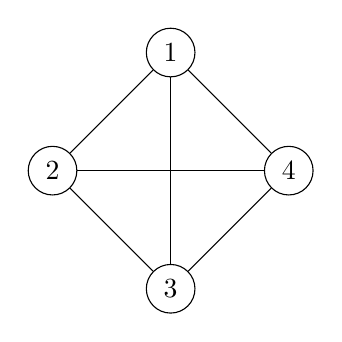
\begin{tikzpicture}[scale=1, every node/.style={circle, draw, fill=white, minimum size=0.6cm}]
  \foreach \k in {1,...,4} {
    \node (v\k) at ({90+90*(\k-1)}:1.5) {\k};
  }
  \foreach \k in {1,...,4} {
    \foreach \l in {1,...,4} {
      \ifnum\k<\l
        \draw (v\k) -- (v\l);
      \fi
    }
  }
\end{tikzpicture}
\end{center}

\item \textbf{Ciclos} ($C_n$): Un ciclo de $n \geq 3$ vértices $v_1,v_2,\dots,v_n$ es aquel grafo simple que contiene las aristas
$\{(v_1,v_2),(v_2,v_3),\dots,(v_{n-1},v_n),(v_n,v_1)\}$. Usamos $C_n$ para denotar al ciclo de $n$ vértices.

\begin{center}
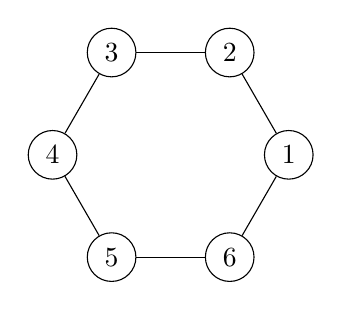
\begin{tikzpicture}[scale=1, every node/.style={circle, draw, fill=white, minimum size=0.6cm}]
  \foreach \k in {1,...,6} {
    \node (v\k) at ({60*(\k-1)}:1.5) {\k};
  }
\foreach \i in {1,...,6} {
  \pgfmathtruncatemacro{\j}{mod(\i,6)+1}
  \draw (v\i) -- (v\j);
}
\end{tikzpicture}
\end{center}

\item \textbf{Grafos bipartitos}: Un grafo $G=(V,E)$ es bipartito sii $V$ puede ser particionado en dos conjuntos $V_1$ y $V_2$ tal que cada arco del grafo conecta un
nodo de $V_1$ con uno de $V_2$, y no hay arcos dentro de un mismo conjunto.conjuntos.

\begin{center}
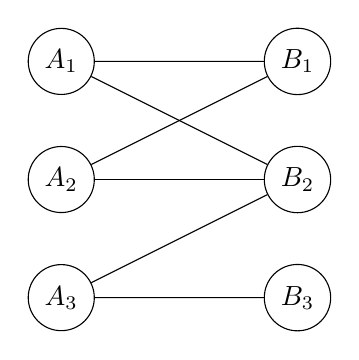
\begin{tikzpicture}[scale=1.5, every node/.style={circle, draw, fill=white, minimum size=0.5cm}]
  \foreach \i in {1,...,3} {
    \node (a\i) at (0,2-\i) {$A_\i$};
    \node (b\i) at (2,2-\i) {$B_\i$};
    \draw (a\i) -- (b\i);
  }
  \draw (a1) -- (b2);
  \draw (a2) -- (b1);
  \draw (a3) -- (b2);
\end{tikzpicture}
\end{center}


\item \textbf{Grafos bipartitos completos} ($K_{m,n}$): Un grafo bipartito se dice además \textbf{completo} si existe un arco entre
\emph{cada} par de nodos $(u,v)$ tal que $u \in V_1$ y $v \in V_2$. Usamos
$K_{|V_1|,|V_2|}$ para denotar a dicho grafo. 

\begin{center}
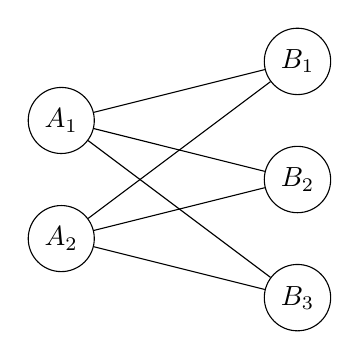
\begin{tikzpicture}[scale=1.5, every node/.style={circle, draw, fill=white, minimum size=0.6cm}]
  \foreach \k in {1,...,2} {
    \node (a\k) at (0,2-\k) {$A_\k$};
  }
  \foreach \l in {1,...,3} {
    \node (b\l) at (2,2.5-\l) {$B_\l$};
  }
  \foreach \k in {1,...,2} {
    \foreach \l in {1,...,3} {
      \draw (a\k) -- (b\l);
    }
  }
\end{tikzpicture}
\end{center}

\end{itemize}


\begin{thmblock}{Caracterización de grafos bipartitos}
Un grafo simple es bipartito si y solo si sus vértices pueden colorearse con dos colores de forma que ningún par de nodos adyacentes tenga el mismo color.
\end{thmblock}
\begin{proof}
($\Rightarrow$) Suponga que $G = (V, E)$ es bipartito y que la partición de $V$ está dada por $V_1$ y $V_2$. Pinte los vértices en $V_1$ de azul y los vértices en $V_2$ de rojo. Como en un grafo bipartito todas las aristas conectan vértices de conjuntos distintos, ningún par de vértices adyacentes estará pintado del mismo color.

\medskip

($\Leftarrow$) Suponga ahora que es posible pintar de rojo o azul cada vértice de $G$ de tal forma que si dos nodos son adyacentes, entonces reciben colores distintos. Defina $V_1$ como el conjunto de nodos coloreados de azul y $V_2$ como el conjunto de nodos coloreados de rojo. Entonces $V = V_1 \cup V_2$ y toda arista conecta un nodo de $V_1$ con uno de $V_2$, lo que demuestra que $G$ es bipartito.
\end{proof}



\subsection{Ejercicios Propuestos}
\begin{enumerate}
\item Use el teorema anterior para determinar si los siguientes grafos son
bipartitos:
\begin{center}
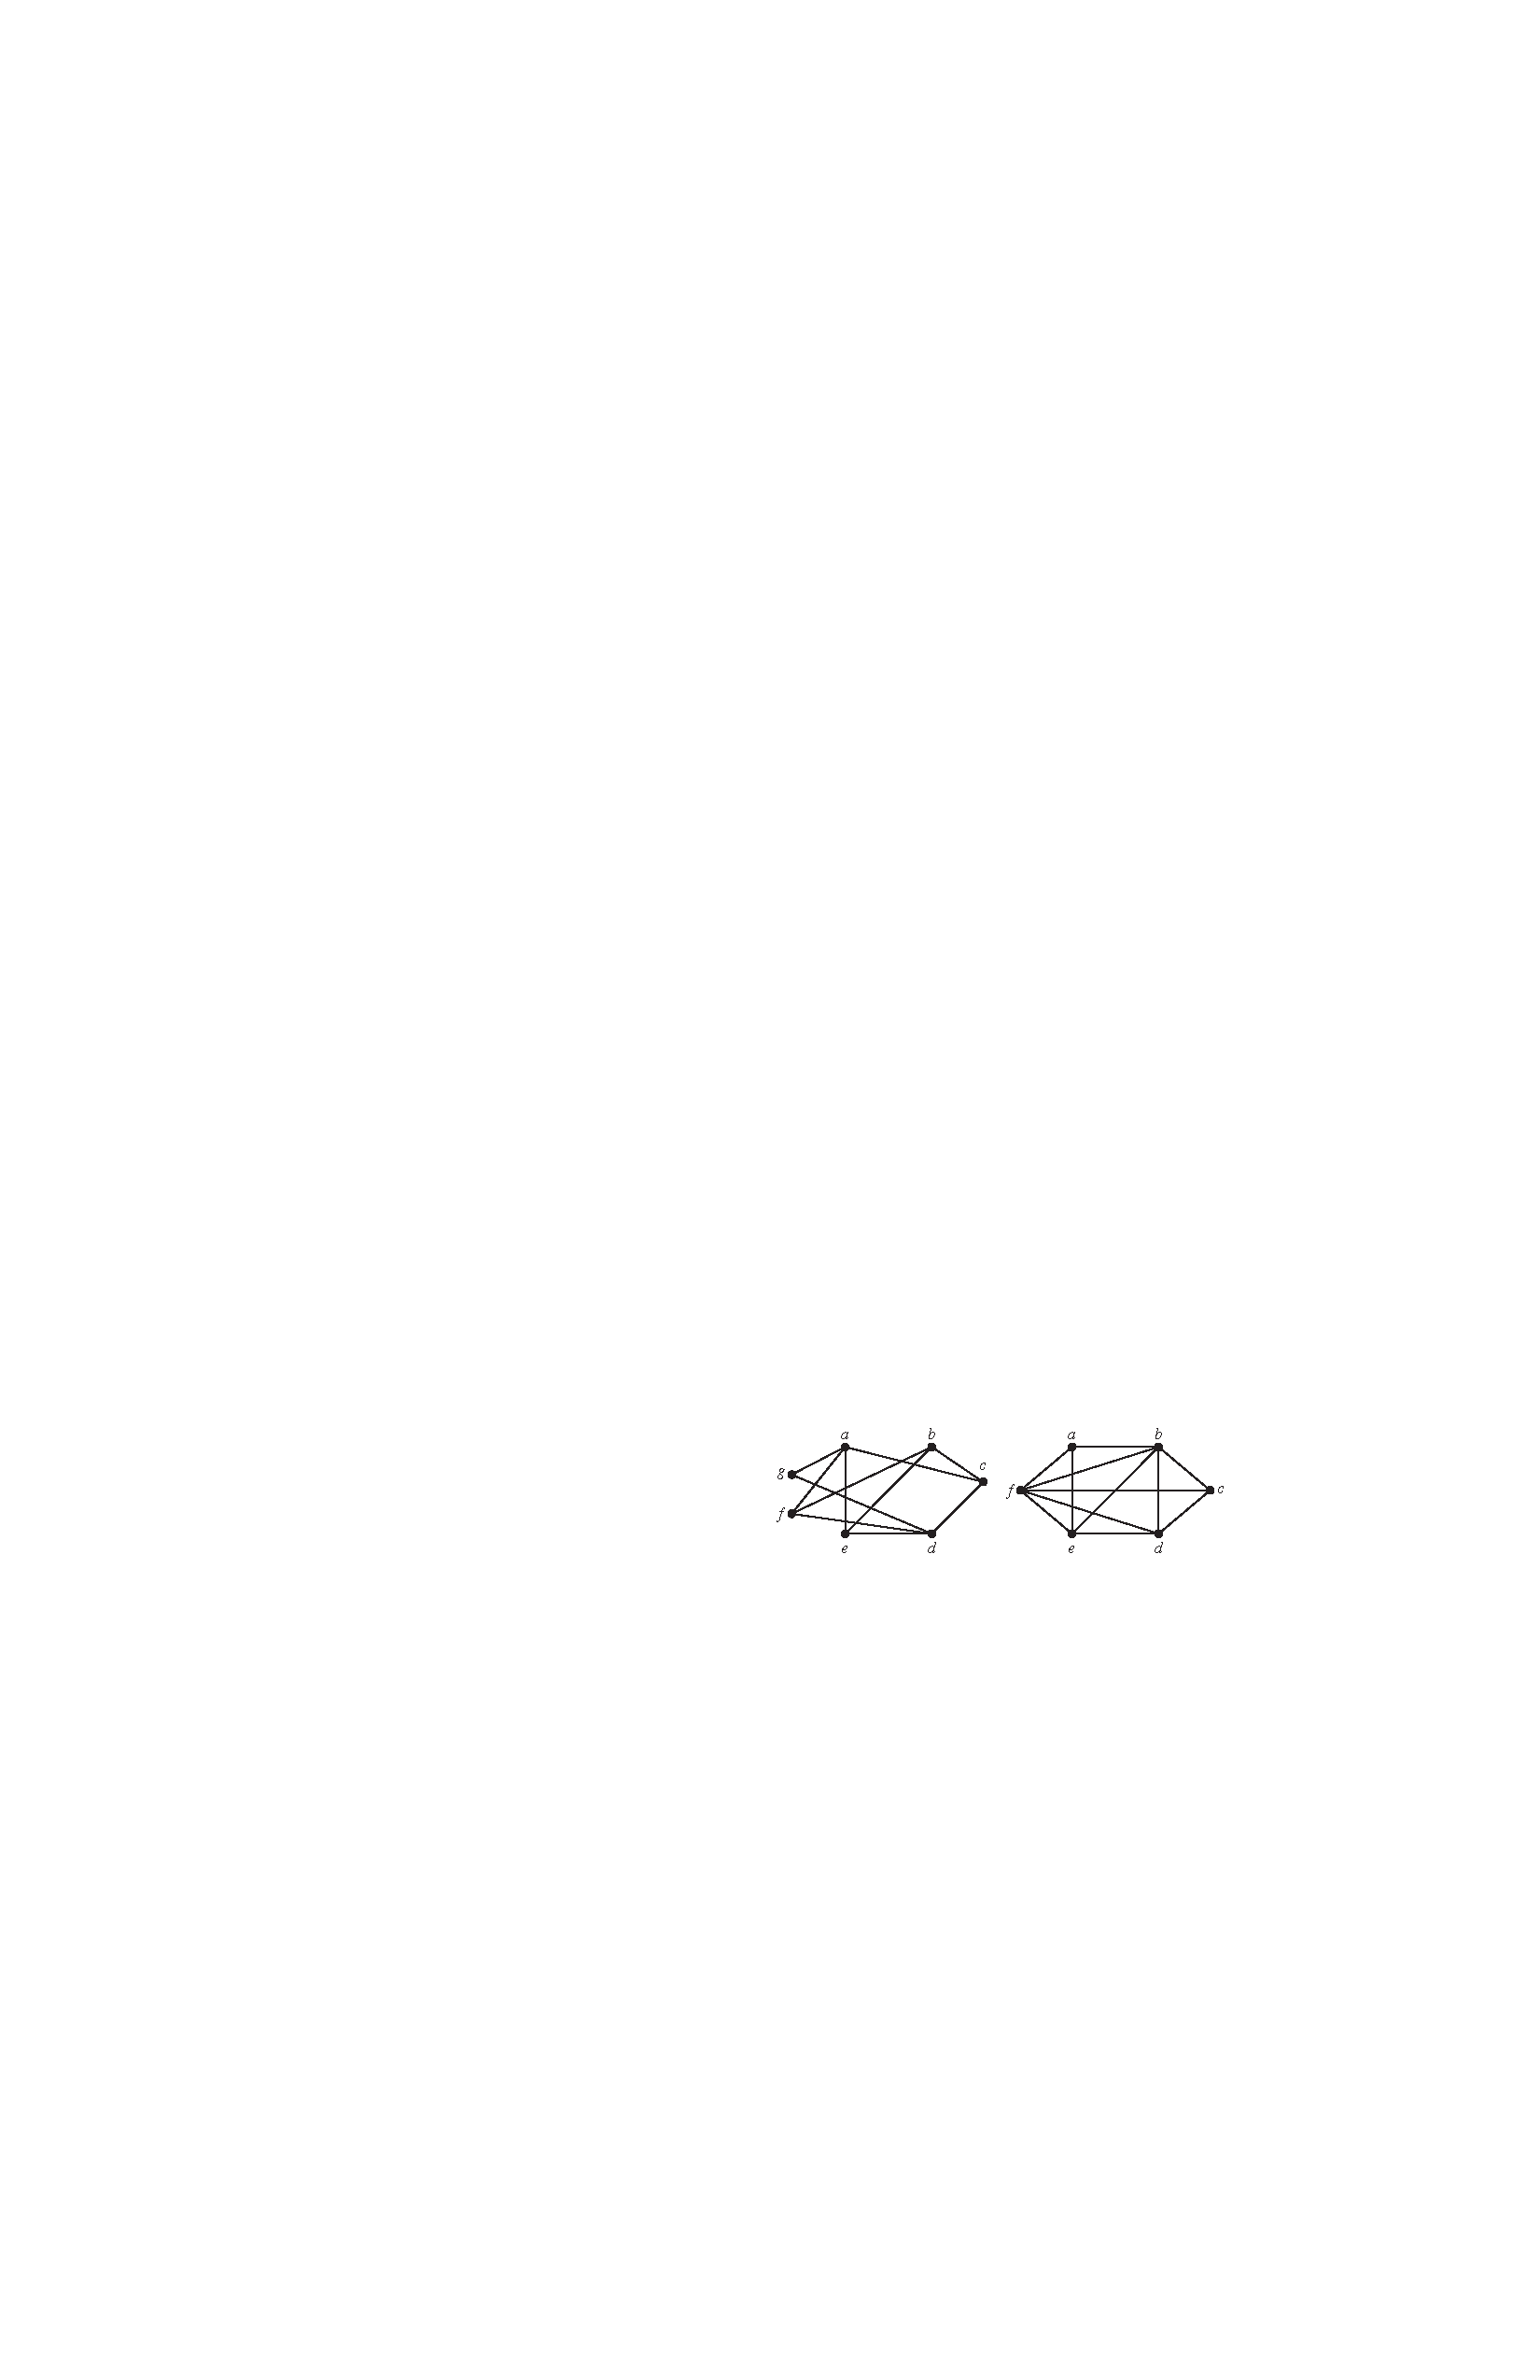
\includegraphics[width=0.7\textwidth]{Figures/ExerciseBipartite.pdf}
\end{center}
\item Demuestre que el ciclo $C_n$ es bipartito si y solo si $n$ es par.
\item Sea $G = (V,E)$ un grafo simple. Demuestre que $$ \min\,\{deg(v) \mid v \in V\} ~\leq~ \frac{2 \, |E|}{|V|} ~\leq~\max\, \{deg(v) \mid v \in V\}$$
\item  Sea $G = (V,E)$ un grafo bipartito simple. Demuestre que 
$|E| \leq |V|^2 / 4$. 
\end{enumerate}









